\documentclass[12pt, a4paper]{article}

% for changing title styles
\usepackage{titlesec}
% sensible margins
\usepackage[margin=1.0in]{geometry}
% include images
\usepackage{graphicx}
% images subcaption
\usepackage{subcaption}
% for maths equations
\usepackage{amsmath}
% for images
\usepackage{graphicx}
% something that everyone includes no idea why
\usepackage[utf8]{inputenc}
% change enumerate numbering styles
\usepackage{enumitem}
% table line
\usepackage{makecell}
% another table stuff
\usepackage{tabularx}
		\newcolumntype{L}{>{\raggedright\arraybackslash}X}
\usepackage{float}

% section spacing
\titlespacing{\section} {12pt} {12pt} {12pt}
% subsection spacing
\titlespacing{\subsection} {10pt} {0pt} {0pt}

% paragraph indentations
\setlength{\parskip} {1em}
\renewcommand{\baselinestretch} {1.5}

\begin{document}

% title page
\begin{center}
\Huge{\textbf{Course Management System}} \\
\vspace{1.5cm}
\Large{\textbf{Object Oriented Programming - II}} \\
\Large{\textbf{Project Dataflow}} \\
\vspace{5mm}
\large{\textbf{\textit{Submitted by}}}
\vspace{5mm}
\end{center}

% Mentioning the authors
\begin{center}
\begin{minipage}{0.30\textwidth}
		\begin{center}
				Abhik Jain \\
				1st Year CSE \\
				(Roll No. 191000001)
		\end{center}
\end{minipage}
\begin{minipage}{0.30\textwidth}
		\begin{center}
				Ayush Mehar \\
				1st Year CSE \\
				(Roll No. 191000011)
		\end{center}
\end{minipage}
\begin{minipage}{0.30\textwidth}
		\begin{center}
				Ishan Kumar Kaler\\
				1st Year CSE \\
				(Roll No. 191000018)
		\end{center}
\end{minipage}
\end{center}

\vspace{1.5cm}

% college logo
\begin{center}
	
\includegraphics[width=4cm]{figures/download.png} \\
\Large{\textbf{Dr. Shyama Prasad Mukherjee\\International Institute of Information Technology\\Naya Raipur}} \\
\vspace{2.5cm}
\Large{\textbf{3\textsuperscript{th} September, 2020}} \\
\end{center}

\newpage

% index
\tableofcontents

\newpage

\section{The GUI}

\begin{figure*}[h]
	\centering
	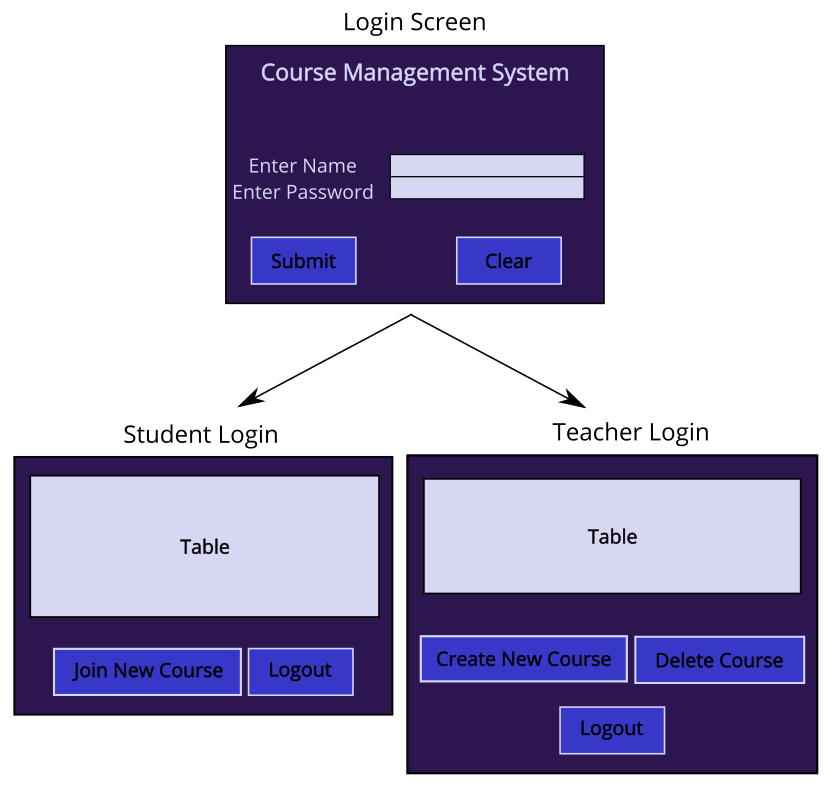
\includegraphics[width=15cm]{figures/gui1.png}
\end{figure*}

The GUI part of the application will be built using Swing library.
When running the application, the user will be greeted by a login screen, Based on the Name and Password input, either the teacher's of student's home screen will be opened.

It'll contain JLabels for heading and to tell user about the fields. JTextField will be used for name and JPasswordField will be used for password input respectively. It'll also have JButtons for login and clear options.

Information from database will be used to check whether password matches of not, and JOptionPane will be used to inform user in case of wrong password or username.

\subsection{Student Home}

When a student will login, his/her info will be retrieved from database and displayed onto the JTable using tableModel. From here, student and select particular course to get more detailed information about a particular course he/she is registered in.

It will contain the option to join new course, for which a new JFrame, which contains a JTable showing all the course the student can join.

We also have the logout option as JButton, which will take us back to Login Screen JFrame and close all other JFrames.

\subsection{Teacher Home}

When a teacher/professor logins, this will be displayed. The JTable contains all the courses the teacher is currently running, and can select any one to view more information about it.

It also contains option to add new courses, which will open new JFrame where a form can be filled to add a new course, as well as option to delete courses. It also has a logout button, similiar to one in Student Home frame.

\section{Database Management}

The database we will be using is SQLite, as it allows one to easily access and share database in file format. The following tables (with fields) will be created and used:

\newpage

\begin{table}[h]
	\centering
	\label{tab:student}
	\begin{tabular}{ c|c }
		\textbf{Field}	& \textbf{Data Type} \\
		\hline
		ID				& integer \\
		name 			& text \\
		password		& integer \\
		join\_year		& integer \\
		courses			& text (course IDs as comma seperated)
	\end{tabular}
	\caption{Student Table}
\end{table}
\vspace*{2.5cm}

\begin{table}[h]
	\centering
	\label{tab:teacher}
	\begin{tabular}{ c|c }
		\textbf{Field}	& \textbf{Data Type} \\
		\hline
		ID				& integer \\
		name 			& text \\
		password		& integer \\
		courses			& text (course IDs as comma seperated)
	\end{tabular}
	\caption{Teacher Table}
\end{table}
\vspace*{2.5cm}

\begin{table}[h]
	\centering
	\label{tab:courses}
	\begin{tabular}{ c|c }
		\textbf{Field}	& \textbf{Data Type} \\
		\hline
		ID				& integer \\
		name 			& text \\
		professor		& integer \\
		prereq			& text \\
		duration 		& int (days) \\
		students 		& text (student IDs as comma seperated)
	\end{tabular}
	\caption{Courses Table}
\end{table}

\newpage

\section{Work Distribution}

\begin{itemize}
	\item \textbf{Ishan Kumar Kaler}: Program logic, frame management including adding functionality to JButtons, JTables etc.
	\item \textbf{Ayush Mehar}: Create Swing GUI elements and forms, and initialise all the event listeners needed.
	\item \textbf{Abhik Jain}: Connecting the Java Program with the database, and writing code to query, update and write to database.
\end{itemize}

\end{document}
